\section{Uso de Seções}

A apresentação deve ser dividida em seções. As seções são apresentadas na agenda, e, de preferência, devem variar entre 5 e 7, não sendo menos que 3, e não ultrapassando 9.

Na maioria das apresentações, duas seções são essenciais: introdução e conclusão. Algumas partes da apresentação, mesmo que sendo obrigatória sua presença, não precisam ter seções indicadas, como a Bibliografia e, quando existir, a apresentação do autor, autores ou grupo de pesquisa. A agenda não é um sumário do documento apresentação, mas sim uma divisão da apresentação em etapas.

Cada seção deve possuir uma slide inicial, na forma de título ou de uma versão da agenda onde a versão atual está indicada de alguma forma. Esta transição avisa a audiência que o apresentador está ``mudando de assunto'', e faz com que consiga acompanhá-lo em seu raciocínio. Pouco precisa ser falado nesses slides, a não ser avisar que um assunto acabou e o outro começa, com uma frase do tipo ``Agora que vimos a nossa proposta, vamos ver como ela foi implementada''.


 Um título de seção pode ter vários formatos, a Figura \ref{fig:sectitles} mostra um simples e três variações que experimentei em aulas diferentes. Em especial, a agenda do slide da Figura \ref{fig:stfancy} usa uma \textit{SmartArt} do \textit{Power Point} e permite usar imagens e funciona bem até 5 seções. Tanto esse formato, quanto do da Figura \ref{fig:st3} mostram toda a agenda de alguma forma.

 O \textit{Power Point} também possui um comando (Insert->Zoom) que permite criar automaticamente um slide que indica as seções.

\begin{figure}[htb]
    \centering
    \subfloat[]{
        
\includegraphics[width=0.4\linewidth,frame]{imagens/sec1}
    }
    \subfloat[]{
        
\includegraphics[width=0.4\linewidth,frame]{imagens/valor}
    }\\
    \subfloat[]{
        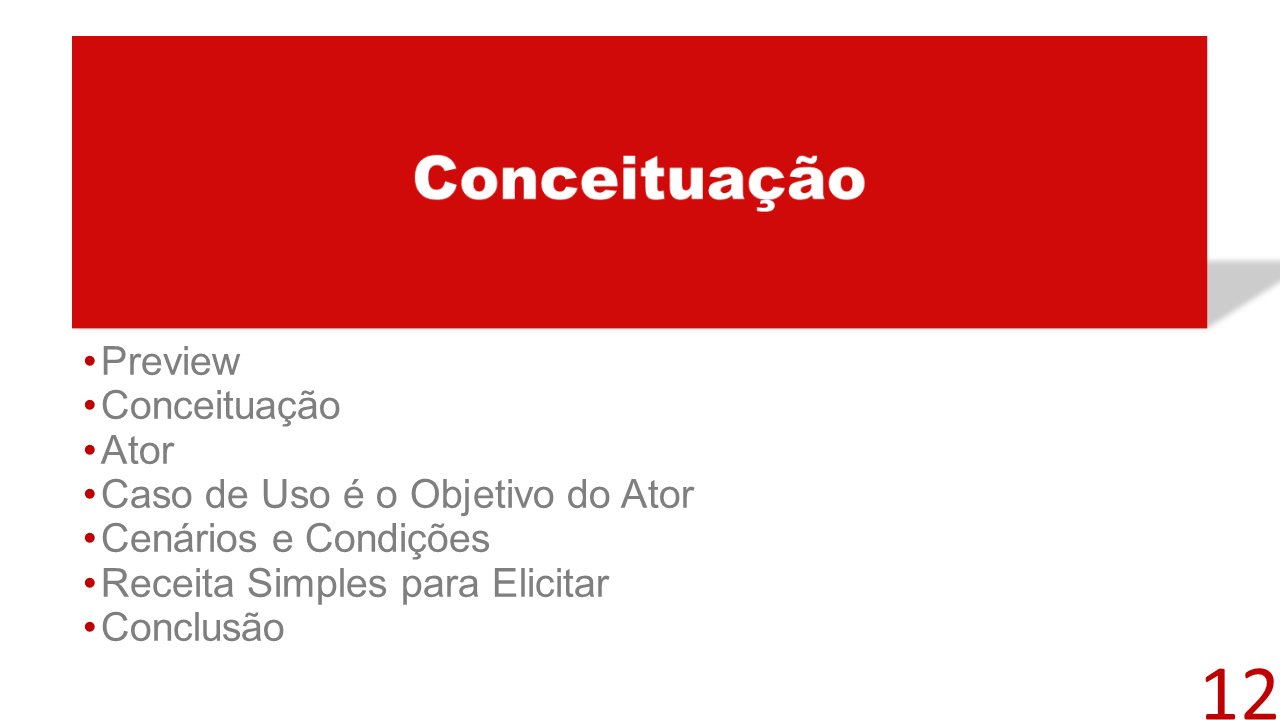
\includegraphics[width=0.4\linewidth,frame]{imagens/casosdeuso}\label{fig:st3}
    }
    \subfloat[]{
        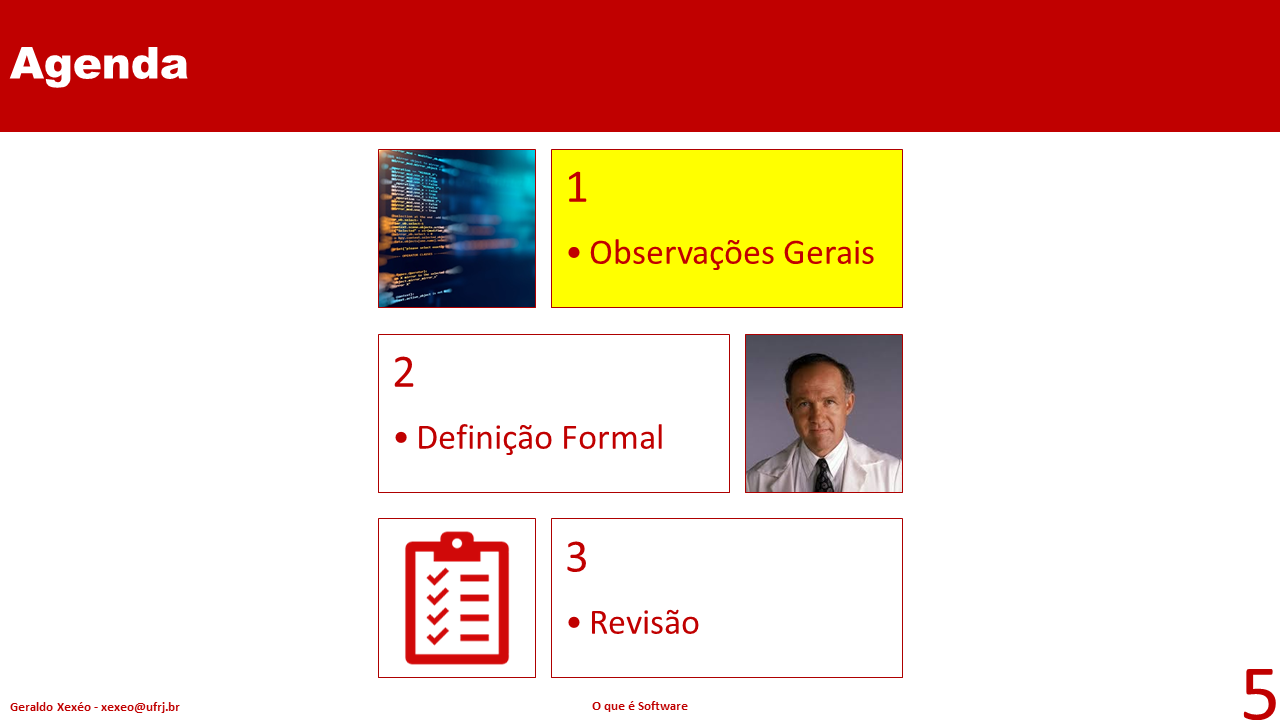
\includegraphics[width=0.4\linewidth,frame]{imagens/sec2}
        \label{fig:stfancy}}
        \caption{Várias formas de fazer um título de seção}.
        \label{fig:sectitles}
    \end{figure}


Os slides que uso para o título da seção lembram os slides de título da apresentação. Essa semelhança não é obrigatória, e talvez devesse ser evitada, apesar de ser \textit{default} no \textit{Power Point}.

\subsection{Processamento de seções no \texttt{beamer}}

 Usado como título de seção, o slide da Figura \ref{fig:meio} mostra um slide com uma versão da agenda levemente modificada por meio do uso de sombra nos itens já tratados, que é criada automaticamente no \texttt{beamer} com os comandos que aparecem na Listagem \ref{lst:autosec}. Esse é um dos poucos usos que aceito para diminuir a intensidade de itens em um slide.

\begin{lstlisting}[language=TeX,caption={Comando para títulos de seção automáticos no \texttt{beamer} com o tema Luebeck.},label={lst:autosec}]
    \AtBeginSection[]
    {\begin{frame}
            \frametitle{Onde Estamos?}
            \tableofcontents[currentsection,hideallsubsections ]
    \end{frame}}
\end{lstlisting}

\begin{figure}[hbt]
    \centering
    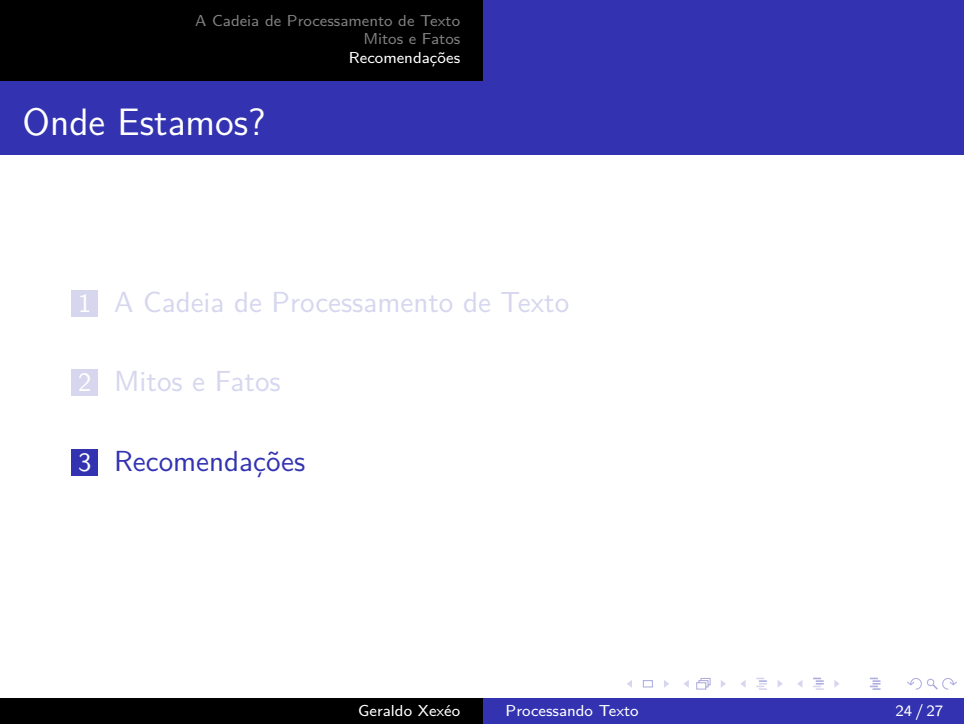
\includegraphics[width=\tam\linewidth,frame]{imagens/agendadomeio.png}
    \caption{Um slide título de seção mostrando a parte que será falada da agenda, com as outras partes acinzentadas. Criada usando o \LaTeX\  e o \texttt{beamer}.}
    \label{fig:meio}
\end{figure}



Para indicar melhor o momento do slide no total da apresentação, o \texttt{beamer} possui alguns temas que geram automaticamente, em cada slide, um índice que mostra o posicionamento do slide na aula. Isso é demonstrado na Figura \ref{fig:sistemas}. No cabeçalho do slide podemos ver o nome da seção e da subseção, que no caso é o mesmo nome do slide\footnote{Essa apresentação, sobre o uso do \LaTeX, está disponível em \url{https://github.com/xexeo/Seminario-LaTeX-2020}}.

\begin{figure}[tbh]
    \centering
    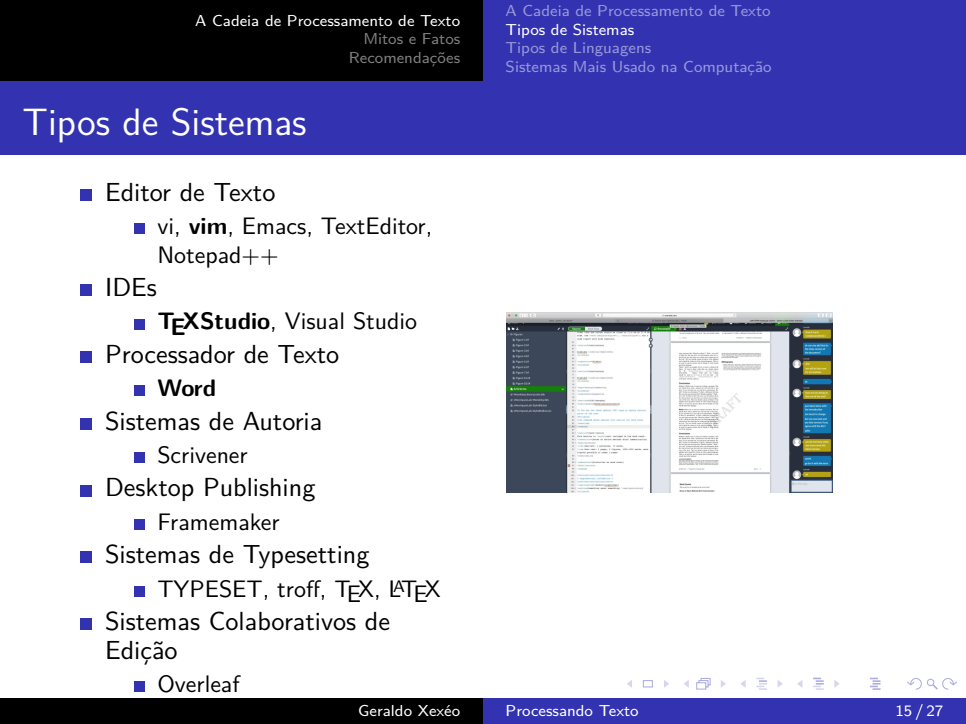
\includegraphics[width=\tam\linewidth,frame]{imagens/sistemas}
    \caption{Slide feito no \texttt{beamer} onde um índice é gerado automaticamente no topo de cada slide com o tema Luebeck}
    \label{fig:sistemas}
\end{figure}


